\begin{appendix}

%------------------------------------------------------------------------------
\chapter{Oracle Data Types}\label{oracle-data-types}
%------------------------------------------------------------------------------
\index{Oracle Data Types}

\section*{Bind Data Types}\label{bind-data-types}

The \inline{oacdty} parameter in a bind variables details determines
the data type of that bind variable. This is not necessarily the data
type of the column in a table that it may be being \inline{INSERT}ed
or \inline{UPDATE}d into, or compared against in a \inline{WHERE} clause.

There is a table of data types and codes in the \emph{Internal Data Types} section
of the \emph{Data Types} chapter in the 12cR2 
\href{http://docs.oracle.com/database/122/LNOCI/data-types.htm\#LNOCI16266}{\emph{Oracle Call
Interface} manual}.

However, various other sources on the internet, and in books, seem to
disagree with some of what the above table shows. In addition, I have
come across many Oracle Trace files where a ROWID was code 11 and not
code 69. Consistency? Who mentioned consistency?

There is, however, a slightly less easy manner of getting the correct data type codes, straight from the horse's mouth. In Oracle 11g this is a view named \inline{DBA\_TAB\_COLS}, while in 12c, it has been renamed to \inline{DBA\_TAB\_COLS\_V\$}. Looking at the source of that view, we can see the following data type codes are in use:

\begin{longtable}[]{@{}r|l@{}}
\toprule
Code & Data Type  \\
\midrule
\endhead
\bottomrule
\caption{Bind Variable data Types\ldots{}\textit{continues on next page}}
\endfoot
\caption{Bind Variable data Types}
\endlastfoot

1 & NVARCHAR2 or VARCHAR2 \\
2 & NUMBER or FLOAT(precision) \\
8 & LONG \\
9 & NCHAR VARYING or VARCHAR \\
12 & DATE \\
23 & RAW \\
24 & LONG RAW \\
58 & ANYDATA or XMLTYPE \\
69 & ROWID \\
96 & NCHAR or CHAR \\
100 & BINARY\_FLOAT \\
101 & BINARY\_DOUBLE \\
105 & MLSLABEL \\
106 & MLSLABEL \\
111 & REF XMLTYPE \\
112 & NCLOB or CLOB \\
113 & BLOB \\
114 & BFILE \\
115 & CFILE \\
121 & User defined and/or object TYPEs \\
122 & User defined and/or object TYPEs \\
123 & User defined and/or object TYPEs \\
178 & TIME(scale) \\
179 & TIME(scale) WITH TIME ZONE \\
180 & TIMESTAMP(scale) \\
181 & TIMESTAMP(scale) WITH TIME ZONE \\
182 & INTERVAL YEAR(precision) TO MONTH \\
183 & INTERVAL DAY(precision) TO SECOND(scale) \\
208 & UROWID (Universal ROWID)\\
231 & TIMESTAMP(scale) WITH LOCAL TIME ZONE \\

\bottomrule
\end{longtable}

\begin{note}
Data types 178 and 179 are both listed in 11g and 12c, but you try creating a table with the \inline{TIME(n)} or \inline{TIME(n) WITH TIME ZONE} and see what happens! They \emph{appear} to be Java data types as that appears to be the only manual that lists them as valid data types.
\end{note}

Anything else, not mentioned above, is \emph{supposedly} an UNDEFINED and/or UNHANDLED data type, however, I have also seen the following in various trace files:

\begin{longtable}[]{@{}r|l@{}}
\toprule
Code & Data Type  \\
\midrule
\endhead
\bottomrule
\caption{Unlisted Bind Data Types\ldots{}\textit{continues on next page}}
\endfoot
\caption{Unlisted Bind Data Types}
\endlastfoot

11 & ROWID \\
102 & REF\_CURSOR \\
108 & User defined TYPEs \\
123 & VARRAY \\

\bottomrule
\end{longtable}

For example, here is a \inline{ROWID} with \inline{oacdty=11} as opposed to \inline{oacdty=69}. The following example was taken from a trace file, created on Windows with Oracle 11.2.0.4:

\begin{lstlisting}[numbers=none,caption={Bind Example - \inline{ROWID} With \inline{oacdty=11}}]
PARSING IN CURSOR #5141169152 len=37 dep=1 uid=0 oct=3 lid=0 tim=3520788504344 hv=1398610540 ad='7ffc0a95d898' sqlid='grwydz59pu6mc'
select text from view$ where rowid=:1
END OF STMT
PARSE #5141169152:c=0,e=14640,p=0,cr=29,cu=0,mis=1,r=0,dep=1,og=4,plh=0,tim=3520788504343
BINDS #5141169152:
 Bind#0
  oacdty=11 mxl=16(16) mxlc=00 mal=00 scl=00 pre=00
  oacflg=18 fl2=0001 frm=00 csi=00 siz=16 off=0
  kxsbbbfp=bff30890  bln=16  avl=16  flg=05
  value=00002787.000A.0001
\end{lstlisting}  
  
There's an example of a \inline{REF\_CURSOR} bind on page \pageref{ref-cursor-102} of this eBook showing the use of an \inline{oacdty=102}.

%------------------------------------------------------------------------------
\chapter{Oracle Command Codes}\label{oracle-command-codes}
%------------------------------------------------------------------------------
\index{Oracle Command Codes}

\section*{Command Codes}\label{command-codes}

The \inline{oct} parameter in a \inline{PARSING IN CURSOR} line in an Oracle
trace file, determines the command that is being parsed in the SQL
statement. Why we should need this, I have no idea, as the SQL text for the
command will - obviously - show what command is being parsed. However\ldots{}

The following (large) table outlines the various command codes and was extracted
from an Oracle 12.1.0.2 database.

\begin{longtable}[]{@{}rl|rl@{}}
\toprule
Code & Command & Code & Command  \\
\midrule
\endhead
\bottomrule
\caption{Oracle Command Codes\ldots{}\textit{continues on next page}}
\endfoot
\caption{Oracle Command Codes}
\endlastfoot

0    & UNKNOWN                      & 111 & DROP PUBLIC SYNONYM          \\
1    & CREATE TABLE                 & 112 & CREATE PUBLIC DATABASE LINK  \\
2    & INSERT                       & 113 & DROP PUBLIC DATABASE LINK    \\
3    & SELECT                       & 114 & GRANT ROLE                   \\
4    & CREATE CLUSTER               & 115 & REVOKE ROLE                  \\      
5    & ALTER CLUSTER                & 116 & EXECUTE PROCEDURE            \\
6    & UPDATE                       & 117 & USER COMMENT                 \\
7    & DELETE                       & 118 & ENABLE TRIGGER               \\
8    & DROP CLUSTER                 & 119 & DISABLE TRIGGER              \\
9    & CREATE INDEX                 & 120 & ENABLE ALL TRIGGERS          \\
10   & DROP INDEX                   & 121 & DISABLE ALL TRIGGERS         \\
11   & ALTER INDEX                  & 122 & NETWORK ERROR                \\
12   & DROP TABLE                   & 123 & EXECUTE TYPE                 \\
13   & CREATE SEQUENCE              & 128 & FLASHBACK                    \\
14   & ALTER SEQUENCE               & 129 & CREATE SESSION               \\
15   & ALTER TABLE                  & 130 & ALTER MINING MODEL           \\
16   & DROP SEQUENCE                & 131 & SELECT MINING MODEL          \\
17   & GRANT OBJECT                 & 133 & CREATE MINING MODEL          \\
18   & REVOKE OBJECT                & 134 & ALTER PUBLIC SYNONYM         \\
19   & CREATE SYNONYM               & 135 & DIRECTORY EXECUTE            \\
20   & DROP SYNONYM                 & 136 & SQL*LOADER DIRECT PATH LOAD  \\
21   & CREATE VIEW                  & 137 & DATAPUMP DIRECT PATH UNLOAD  \\
22   & DROP VIEW                    & 138 & DATABASE STARTUP             \\
23   & VALIDATE INDEX               & 139 & DATABASE SHUTDOWN            \\
24   & CREATE PROCEDURE             & 140 & CREATE SQL TXLN PROFILE      \\
25   & ALTER PROCEDURE              & 141 & ALTER SQL TXLN PROFILE       \\
26   & LOCK                         & 142 & USE SQL TXLN PROFILE         \\
27   & NO-OP                        & 143 & DROP SQL TXLN PROFILE        \\
28   & RENAME                       & 144 & CREATE MEASURE FOLDER        \\
29   & COMMENT                      & 145 & ALTER MEASURE FOLDER         \\
30   & AUDIT OBJECT                 & 146 & DROP MEASURE FOLDER          \\
31   & NOAUDIT OBJECT               & 147 & CREATE CUBE BUILD PROCESS    \\
32   & CREATE DATABASE LINK         & 148 & ALTER CUBE BUILD PROCESS     \\
33   & DROP DATABASE LINK           & 149 & DROP CUBE BUILD PROCESS      \\
34   & CREATE DATABASE              & 150 & CREATE CUBE                  \\
35   & ALTER DATABASE               & 151 & ALTER CUBE                   \\
36   & CREATE ROLLBACK SEG          & 152 & DROP CUBE                    \\  
37   & ALTER ROLLBACK SEG           & 153 & CREATE CUBE DIMENSION        \\
38   & DROP ROLLBACK SEG            & 154 & ALTER CUBE DIMENSION         \\
39   & CREATE TABLESPACE            & 155 & DROP CUBE DIMENSION          \\
40   & ALTER TABLESPACE             & 157 & CREATE DIRECTORY             \\
41   & DROP TABLESPACE              & 158 & DROP DIRECTORY               \\
42   & ALTER SESSION                & 159 & CREATE LIBRARY               \\
43   & ALTER USER                   & 160 & CREATE JAVA                  \\
44   & COMMIT                       & 161 & ALTER JAVA                   \\
45   & ROLLBACK                     & 162 & DROP JAVA                    \\
46   & SAVEPOINT                    & 163 & CREATE OPERATOR              \\
47   & PL/SQL EXECUTE               & 164 & CREATE INDEXTYPE             \\
48   & SET TRANSACTION              & 165 & DROP INDEXTYPE               \\
49   & ALTER SYSTEM                 & 166 & ALTER INDEXTYPE              \\
50   & EXPLAIN                      & 167 & DROP OPERATOR                \\
51   & CREATE USER                  & 168 & ASSOCIATE STATISTICS         \\
52   & CREATE ROLE                  & 169 & DISASSOCIATE STATISTICS      \\
53   & DROP USER                    & 170 & CALL METHOD                  \\
54   & DROP ROLE                    & 171 & CREATE SUMMARY               \\
55   & SET ROLE                     & 172 & ALTER SUMMARY                \\
56   & CREATE SCHEMA                & 173 & DROP SUMMARY                 \\
57   & CREATE CONTROL FILE          & 174 & CREATE DIMENSION             \\
59   & CREATE TRIGGER               & 175 & ALTER DIMENSION              \\
60   & ALTER TRIGGER                & 176 & DROP DIMENSION               \\
61   & DROP TRIGGER                 & 177 & CREATE CONTEXT               \\
62   & ANALYZE TABLE                & 178 & DROP CONTEXT                 \\
63   & ANALYZE INDEX                & 179 & ALTER OUTLINE                \\
64   & ANALYZE CLUSTER              & 180 & CREATE OUTLINE               \\
65   & CREATE PROFILE               & 181 & DROP OUTLINE                 \\
66   & DROP PROFILE                 & 182 & UPDATE INDEXES               \\
67   & ALTER PROFILE                & 183 & ALTER OPERATOR               \\
68   & DROP PROCEDURE               & 190 & PASSWORD CHANGE              \\
70   & ALTER RESOURCE COST          & 192 & ALTER SYNONYM                \\
71   & CREATE MATERIALIZED VIEW LOG & 197 & PURGE USER\_RECYCLEBIN       \\
72   & ALTER MATERIALIZED VIEW LOG  & 198 & PURGE DBA\_RECYCLEBIN        \\
73   & DROP MATERIALIZED VIEW LOG   & 199 & PURGE TABLESPACE             \\
74   & CREATE MATERIALIZED VIEW     & 200 & PURGE TABLE                  \\
75   & ALTER MATERIALIZED VIEW      & 201 & PURGE INDEX                  \\
76   & DROP MATERIALIZED VIEW       & 202 & UNDROP OBJECT                \\
77   & CREATE TYPE                  & 204 & FLASHBACK DATABASE           \\
78   & DROP TYPE                    & 205 & FLASHBACK TABLE              \\
79   & ALTER ROLE                   & 206 & CREATE RESTORE POINT         \\
80   & ALTER TYPE                   & 207 & DROP RESTORE POINT           \\
81   & CREATE TYPE BODY             & 208 & PROXY AUTHENTICATION ONLY    \\
82   & ALTER TYPE BODY              & 209 & DECLARE REWRITE EQUIVALENCE  \\
83   & DROP TYPE BODY               & 210 & ALTER REWRITE EQUIVALENCE    \\
84   & DROP LIBRARY                 & 211 & DROP REWRITE EQUIVALENCE     \\
85   & TRUNCATE TABLE               & 212 & CREATE EDITION               \\
86   & TRUNCATE CLUSTER             & 213 & ALTER EDITION                \\
88   & ALTER VIEW                   & 214 & DROP EDITION                 \\
91   & CREATE FUNCTION              & 215 & DROP ASSEMBLY                \\
92   & ALTER FUNCTION               & 216 & CREATE ASSEMBLY              \\
93   & DROP FUNCTION                & 217 & ALTER ASSEMBLY               \\
94   & CREATE PACKAGE               & 218 & CREATE FLASHBACK ARCHIVE     \\
95   & ALTER PACKAGE                & 219 & ALTER FLASHBACK ARCHIVE      \\
96   & DROP PACKAGE                 & 220 & DROP FLASHBACK ARCHIVE       \\
97   & CREATE PACKAGE BODY          & 225 & ALTER DATABASE LINK          \\
98   & ALTER PACKAGE BODY           & 226 & CREATE PLUGGABLE DATABASE    \\
99   & DROP PACKAGE BODY            & 227 & ALTER PLUGGABLE DATABASE     \\
100  & LOGON                        & 228 & DROP PLUGGABLE DATABASE      \\
101  & LOGOFF                       & 229 & CREATE AUDIT POLICY          \\
102  & LOGOFF BY CLEANUP            & 230 & ALTER AUDIT POLICY           \\
103  & SESSION REC                  & 231 & DROP AUDIT POLICY            \\
104  & SYSTEM AUDIT                 & 232 & CODE-BASED GRANT             \\
105  & SYSTEM NOAUDIT               & 233 & CODE-BASED REVOKE            \\
106  & AUDIT DEFAULT                & 238 & ADMINISTER KEY MANAGEMENT    \\
107  & NOAUDIT DEFAULT              & 239 & CREATE MATERIALIZED ZONEMAP  \\
108  & SYSTEM GRANT                 & 240 & ALTER MATERIALIZED ZONEMAP   \\
109  & SYSTEM REVOKE                & 241 & DROP MATERIALIZED ZONEMAP    \\
110  & CREATE PUBLIC SYNONYM        & 305 & ALTER PUBLIC DATABASE LINK   \\

\bottomrule
\end{longtable}

The exact list of commands for your particular database version can be
extracted using the following SQL command:

\begin{lstlisting}[language=SQL,caption={SQL Query to List Oracle Command Codes}]
select action as code,
       name as command
from   audit_actions;
\end{lstlisting}

There are 212 different commands in Oracle 12c (12.1.0.2) while Oracle
11g (11.2.0.4) has only (!) 181.

%------------------------------------------------------------------------------
\chapter{Oracle Characterset Codes}\label{oracle-characterset-codes}
%------------------------------------------------------------------------------
\index{Oracle Character Set Codes}

\section*{Bind Charactersets}\label{bind-charactersets}

Some data types use different character sets. These are coded in the \inline{csi} field in the bind details lines of the trace file. You can extract the list of current character set codes and names with the following query:

\begin{lstlisting}[language=SQL,caption={SQL Query to list Character Set Codes and Names}]
select nls_charset_id(value), value 
from   v$nls_valid_values
where  isdeprecated='FALSE'
and    parameter = 'CHARACTERSET'
order  by nls_charset_id(value);
\end{lstlisting}

The values that you may see here are as follows, taken from an Oracle 12.1.0.1 database where there are 222 character sets listed:


\begin{longtable}[]{@{}rl|rl|rl@{}}
\toprule
Code & Character Set & Code & Character Set & Code & Character Set \\
\midrule
\endhead
\bottomrule
\caption{Oracle Character Set Codes\ldots{}\textit{continues on next page}}
\endfoot
\caption{Oracle Character Set Codes}
\endlastfoot

1   & US7ASCII       & 159 & CL8MACCYRILLICS   & 301  & EE8EBCDIC870C    \\
2   & WE8DEC         & 160 & WE8PC860          & 312  & TR8EBCDIC1026S   \\
3   & WE8HP          & 161 & IS8PC861          & 314  & BLT8EBCDIC1112S  \\
4   & US8PC437       & 162 & EE8MACCES         & 315  & IW8EBCDIC424S    \\
5   & WE8EBCDIC37    & 163 & EE8MACCROATIANS   & 316  & EE8EBCDIC870S    \\
6   & WE8EBCDIC500   & 164 & TR8MACTURKISHS    & 317  & CL8EBCDIC1025S   \\
7   & WE8EBCDIC1140  & 165 & IS8MACICELANDICS  & 319  & TH8TISEBCDICS    \\
8   & WE8EBCDIC285   & 166 & EL8MACGREEKS      & 320  & AR8EBCDIC420S    \\
9   & WE8EBCDIC1146  & 167 & IW8MACHEBREWS     & 322  & CL8EBCDIC1025C   \\
10  & WE8PC850       & 170 & EE8MSWIN1250      & 323  & CL8EBCDIC1025R   \\
11  & D7DEC          & 171 & CL8MSWIN1251      & 324  & EL8EBCDIC875R    \\
12  & F7DEC          & 172 & ET8MSWIN923       & 325  & CL8EBCDIC1158    \\
13  & S7DEC          & 173 & BG8MSWIN          & 326  & CL8EBCDIC1158R   \\
14  & E7DEC          & 174 & EL8MSWIN1253      & 327  & EL8EBCDIC423R    \\
15  & SF7ASCII       & 175 & IW8MSWIN1255      & 351  & WE8MACROMAN8     \\
16  & NDK7DEC        & 176 & LT8MSWIN921       & 352  & WE8MACROMAN8S    \\
17  & I7DEC          & 177 & TR8MSWIN1254      & 353  & TH8MACTHAI       \\
18  & NL7DEC         & 178 & WE8MSWIN1252      & 354  & TH8MACTHAIS      \\
19  & CH7DEC         & 179 & BLT8MSWIN1257     & 368  & HU8CWI2          \\
20  & YUG7ASCII      & 180 & D8EBCDIC273       & 380  & EL8PC437S        \\
21  & SF7DEC         & 181 & I8EBCDIC280       & 381  & EL8EBCDIC875     \\
22  & TR7DEC         & 182 & DK8EBCDIC277      & 382  & EL8PC737         \\
23  & IW7IS960       & 183 & S8EBCDIC278       & 383  & LT8PC772         \\
25  & IN8ISCII       & 184 & EE8EBCDIC870      & 384  & LT8PC774         \\
27  & WE8EBCDIC1148  & 185 & CL8EBCDIC1025     & 385  & EL8PC869         \\
28  & WE8PC858       & 186 & F8EBCDIC297       & 386  & EL8PC851         \\
31  & WE8ISO8859P1   & 187 & IW8EBCDIC1086     & 390  & CDN8PC863        \\
32  & EE8ISO8859P2   & 188 & CL8EBCDIC1025X    & 401  & HU8ABMOD         \\
33  & SE8ISO8859P3   & 189 & D8EBCDIC1141      & 500  & AR8ASMO8X        \\
34  & NEE8ISO8859P4  & 190 & N8PC865           & 554  & AR8NAFITHA711    \\
35  & CL8ISO8859P5   & 191 & BLT8CP921         & 555  & AR8SAKHR707      \\
36  & AR8ISO8859P6   & 192 & LV8PC1117         & 556  & AR8MUSSAD768     \\
37  & EL8ISO8859P7   & 193 & LV8PC8LR          & 557  & AR8ADOS710       \\
38  & IW8ISO8859P8   & 194 & BLT8EBCDIC1112    & 558  & AR8ADOS720       \\
39  & WE8ISO8859P9   & 195 & LV8RST104090      & 559  & AR8APTEC715      \\
40  & NE8ISO8859P10  & 196 & CL8KOI8R          & 560  & AR8MSWIN1256     \\
41  & TH8TISASCII    & 197 & BLT8PC775         & 561  & AR8NAFITHA721    \\
42  & TH8TISEBCDIC   & 198 & DK8EBCDIC1142     & 563  & AR8SAKHR706      \\
43  & BN8BSCII       & 199 & S8EBCDIC1143      & 565  & AR8ARABICMAC     \\
44  & VN8VN3         & 200 & I8EBCDIC1144      & 566  & AR8ARABICMACS    \\
45  & VN8MSWIN1258   & 201 & F7SIEMENS9780X    & 590  & LA8ISO6937       \\
46  & WE8ISO8859P15  & 202 & E7SIEMENS9780X    & 829  & JA16VMS          \\
47  & BLT8ISO8859P13 & 203 & S7SIEMENS9780X    & 830  & JA16EUC          \\
48  & CEL8ISO8859P14 & 204 & DK7SIEMENS9780X   & 831  & JA16EUCYEN       \\
49  & CL8ISOIR111    & 205 & N7SIEMENS9780X    & 832  & JA16SJIS         \\
50  & WE8NEXTSTEP    & 206 & I7SIEMENS9780X    & 833  & JA16DBCS         \\
51  & CL8KOI8U       & 207 & D7SIEMENS9780X    & 834  & JA16SJISYEN      \\
52  & AZ8ISO8859P9E  & 208 & F8EBCDIC1147      & 835  & JA16EBCDIC930    \\
70  & AR8EBCDICX     & 210 & WE8GCOS7          & 836  & JA16MACSJIS      \\
81  & EL8DEC         & 211 & EL8GCOS7          & 837  & JA16EUCTILDE     \\
82  & TR8DEC         & 221 & US8BS2000         & 838  & JA16SJISTILDE    \\
90  & WE8EBCDIC37C   & 222 & D8BS2000          & 840  & KO16KSC5601      \\
91  & WE8EBCDIC500C  & 223 & F8BS2000          & 842  & KO16DBCS         \\
92  & IW8EBCDIC424   & 224 & E8BS2000          & 845  & KO16KSCCS        \\
93  & TR8EBCDIC1026  & 225 & DK8BS2000         & 846  & KO16MSWIN949     \\
94  & WE8EBCDIC871   & 226 & S8BS2000          & 850  & ZHS16CGB231280   \\
95  & WE8EBCDIC284   & 230 & WE8BS2000E        & 851  & ZHS16MACCGB23128 \\
96  & WE8EBCDIC1047  & 231 & WE8BS2000         & 852  & ZHS16GBK        \\
97  & WE8EBCDIC1140C & 232 & EE8BS2000         & 853  & ZHS16DBCS       \\
98  & WE8EBCDIC1145  & 233 & CE8BS2000         & 854  & ZHS32GB18030    \\
99  & WE8EBCDIC1148C & 235 & CL8BS2000         & 860  & ZHT32EUC        \\
100 & WE8EBCDIC1047E & 239 & WE8BS2000L5       & 861  & ZHT32SOPS       \\
101 & WE8EBCDIC924   & 241 & WE8DG             & 862  & ZHT16DBT        \\
110 & EEC8EUROASCI   & 251 & WE8NCR4970        & 863  & ZHT32TRIS       \\
113 & EEC8EUROPA3    & 261 & WE8ROMAN8         & 864  & ZHT16DBCS       \\
114 & LA8PASSPORT    & 262 & EE8MACCE          & 865  & ZHT16BIG5       \\
140 & BG8PC437S      & 263 & EE8MACCROATIAN    & 866  & ZHT16CCDC       \\
150 & EE8PC852       & 264 & TR8MACTURKISH     & 867  & ZHT16MSWIN950   \\
152 & RU8PC866       & 265 & IS8MACICELANDIC   & 868  & ZHT16HKSCS      \\
153 & RU8BESTA       & 266 & EL8MACGREEK       & 871  & UTF8            \\
154 & IW8PC1507      & 267 & IW8MACHEBREW      & 872  & UTFE            \\
155 & RU8PC855       & 277 & US8ICL            & 873  & AL32UTF8        \\
156 & TR8PC857       & 278 & WE8ICL            & 992  & ZHT16HKSCS31    \\
158 & CL8MACCYRILLIC & 279 & WE8ISOICLUK       & 2000 & AL16UTF16       \\

\bottomrule
\end{longtable}

If you see a character set code in the \inline{csi} field, and you don't have the above list, you can determine the characterset in use with the following query:

\begin{lstlisting}[language=SQL,caption={SQL Query to Convert a \inline{csi} Code to a Charcter Set Name}]
SELECT NLS_CHARSET_NAME(1) FROM dual;
\end{lstlisting}

Correspondingly, you can go from a charcter set name to its \inline{csi} code with the following query:

\begin{lstlisting}[language=SQL,caption={SQL Query to Convert a Charcter Set Name  to a \inline{csi} Code}]
SELECT NLS_CHARSET_ID('US7ASCII') FROM dual;
\end{lstlisting}

%------------------------------------------------------------------------------
\chapter{How this Book Evolved}
%------------------------------------------------------------------------------
\label{how-this-book-evolved}%

\section{Why this Book?}\label{why-this-book}

This eBook originally started as a collection of useful notes, scripts, etc which I had come across, written or deduced, over the years of playing with Oracle Trace Files and various Trace File Analysis tools.

Eventually, I collected them all together in one place so that I could have all the useful information, in one easy to find place\footnote{I'm getting old, every day it seems. I am starting to forget things I knew - they are ageing out of the cache! I now appear to have the memory capacity of a small newt, so I need to have things written down!}.

There are many places on the internet, people I have met or worked with, books which I have bought (or had bought for me) and read, to whom I will always be grateful as they have taught me many things. Maybe I can help others as I have been helped.

As Isaac Newton\index{Newton, Isaac}\person{Newton, Isaac} is thought to have said, ``\emph{I have stood on the shoulders of giants}'' - me too.


\section{Creating the Book}\label{creating-the-book}

The book was created in plain text files, originally in \href{https://en.wikipedia.org/wiki/ReStructuredText}{ReStructuredText} mode, written (and edited) on both Windows\footnote{At work, in my lunch hour}, or on Linux - which I use for all my personal and business needs at home.

These RST files were simply a quick way to gather notes. They were then later enhanced by adding more detail and/or example code, and converted to \LaTeX{}\program{\LaTeX{}} by judicious use of the \href{https://pandoc.org/}{Pandoc}\program{Pandoc} text conversion utility, which I \emph{highly} recommend.

The converted \LaTeX{}\program{\LaTeX{}} files were then further enhanced, indexed, tidied up, etc using \href{http://www.texstudio.org/}{TexStudio}\program{TexStudio} which runs on both Windows and Linux, so I had the same development environment in both locations. Handy. 

The book itself, was created using a \LaTeX{}\program{\LaTeX{}} template called [the] \href{https://www.latextemplates.com/template/the-legrand-orange-book}{Legrand Orange Book Template} created by Mathias Legrand\index{Legrand, Mathias}. It is thanks to him that you get this book for free, because the licence terms of the book template specify no commercial use. I'm happy with that myself.

The front cover image on this book is taken from the book \emph{Kunstformen der Natur}\index{Kunstformen der Natur} by German biologist Ernst Haeckel\index{Haeckel, Ernst}\person{Haeckel, Ernst}. The book was published between 1899 and 1904. The image used is of various \emph{Discomedusae}\index{Discomedusae} which are a taxonomic group of jellyfish.

You can read about them on \href{https://en.wikipedia.org/wiki/Discomedusae}{Wikipedia} and there is a brief overview of the above book, also on \href{https://en.wikipedia.org/wiki/Kunstformen_der_Natur}{Wikipedia},
which shows a number of other images taken from the book. (Some of which I considered before choosing the current one!)

\emph{Discomedusae}\index{Discomedusae}\footnote{DiscoMedusae? Sounds like dancing jellyfish to me!} have absolutely nothing to do with Oracle or Trace Files - but I liked the image, and decided that it would make a good cover for the book and a decent enough chapter heading image too.

%------------------------------------------------------------------------------
\chapter{TraceAdjust Utility}
%------------------------------------------------------------------------------
\label{traceadjust}\program{TraceAdjust}

\section*{TraceAdjust Introduction}\label{traceadjust-introduction}


\emph{TraceAdjust} is a utility that I wrote to help me process the
myriads of trace files that I come across in my DBA work. You can get
the source code from github in my 
\href{https://github.com/NormanDunbar/TraceAdjust}{TraceAdjust repository} and compile it
on Windows or Linux/Unix with any decent C++ compiler.

It reads a normal trace file and writes out an adjusted one, as follows:

\begin{itemize}
\tightlist
\item
  The \inline{tim} values are converted to seconds, by inserting a
  decimal point in the appropriate position;
\item
  It adds a \inline{delta} to each \inline{tim} line. The delta is
  the number of microseconds between the \inline{tim} on this line,
  and the \inline{tim} on the previous (appropriate) trace line. This
  allows me to see how long passed between the previous \inline{tim}
  and this one. Occasionally useful.
\item
  It adds a \inline{dslt} to each \inline{tim} line. This is the
  ``delta since last timestamp'' and simply counts up the number of
  microseconds that have passed since the trace file last produced a
  timestamp line similar to the one in the header. Again, occasionally
  useful.
\item
  It adds a \inline{local} to each \inline{tim} line. This is a
  conversion of the \inline{tim} value on the line, to an actual
  date, in the current local timezone. The time part is resolved down to
  microsecond level. This is usually very useful!
\end{itemize}

Running a trace file through TraceAdjust\program{TraceAdjust} will create a new trace file,
which some trace analysing utilities cannot cope with due to the
additional fields that I have introduced. The Trace File Browser, in
Toad\program{Toad}, on the other hand, copes with my trace files quite happily and
simply ignores the additional data as appropriate.

The example below shows the before and after state of a \inline{PARSE} line from a trace file:


\begin{lstlisting}[numbers=none,caption={TraceAdjust Example - Before Processing}]
PARSE #4474286416:c=0,e=418,p=0,cr=0,cu=0,mis=1,r=0,dep=1,og=4,plh=0,tim=1030574627220
\end{lstlisting}

Which becomes:

\begin{lstlisting}[numbers=none,caption={TraceAdjust Example - After Processing}]
PARSE #4474286416:c=0,e=418,p=0,cr=0,cu=0,mis=1,r=0,dep=1,og=4,plh=0,tim=1030574.627220,delta=-1,dslt=768371,local='2017 Mar 13 09:23:21.768371'
\end{lstlisting}

%------------------------------------------------------------------------------
\chapter{TraceMiner2 Utility}
%------------------------------------------------------------------------------
\label{traceminer2-utility}
\program{TraceMiner2}

\section*{TraceMiner2 Introduction}\label{traceminer2-introduction}

So, you have a trace file, chock full of statements with lots of bind
variables in use. You \emph{need} to read through it to find out which
execution of any of the statements used which actual bind values. How is
this easily done?

\emph{TraceMiner2}\program{TraceMiner2}\footnote{There will be no more unashamed plugs in this
  document, I promise.} is another utility that I wrote to help me
process the myriads of trace files that I come across in my DBA work.

You can get the source code from github in my 
\href{https://github.com/NormanDunbar/TraceMiner2}{TraceMiner2 repository} and compile it
on Windows or Linux/Unix with any decent C++ compiler.

It reads a trace file and writes out an HTML report showing various
details of the SQL in the file, showing:

\begin{itemize}
\tightlist
\item
  The line number of the file where the SQL statement was found at
  (\inline{PARSING IN CURSOR});
\item
  The line number of the file where  the \inline{PARSE} statement was found at;
\item
  The line number of the file where  the \inline{BINDS} details were found at;
\item
  The line number of the file where  the \inline{EXEC} statement was found at;
\item
  The depth (\inline{dep}) of the statement when parsed etc.
\end{itemize}

You can choose to ignore statements over any given depth, so if you only
want top-level and \inline{dep=1} statements, just request \inline{--depth=1} on the
command line. 

The default HTML report appears as follows:

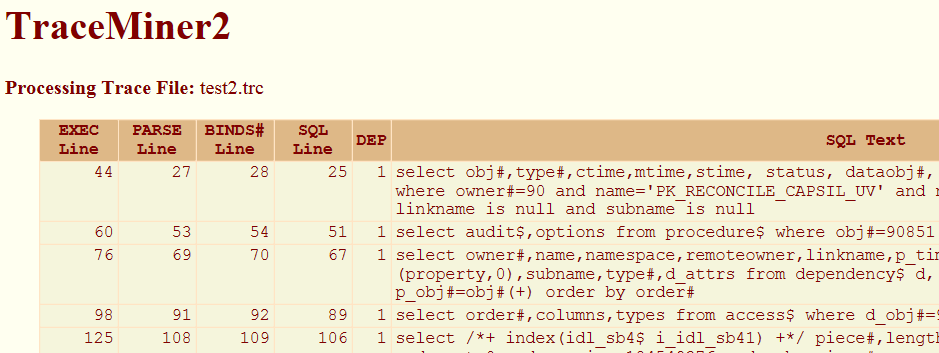
\includegraphics[width=\textwidth]{Content/images/TraceMiner2.png}

However, you can, if you have a standard report format at your company,
configure the generated css file to match that of your format.
\emph{TraceMiner2}\program{TraceMiner2} will not overwrite the css file if one exists in the
output folder.



\end{appendix}
